% Original book diagram: fig:ekf_pf_decision
% Book source: sections/Part_I/RT_bayesian_systems.tex
% Original diagram authorship retained. Visual design: Ziad Mosalam.
\documentclass[11pt,border=8pt]{standalone}
\usepackage{amsmath,amssymb,graphicx,tikz}
\usetikzlibrary{arrows.meta,automata,positioning,calc,shapes.geometric,fit,backgrounds,patterns}
\newcommand{\vect}[1]{\mathbf{#1}}
\newcommand{\mat}[1]{\mathbf{#1}}
\newcommand{\Normal}{\mathcal{N}}
\newcommand{\prob}{p}
\newcommand{\E}{\mathbb{E}}
\newcommand{\Var}{\mathrm{Var}}
\newcommand{\Cov}{\mathrm{Cov}}
\newcommand{\CovP}{\mathbf{P}}
\newcommand{\Prob}{\mathbb{P}}
\setlength{\textwidth}{6.5in}
% Shared visual vocabulary for the book's original diagrams.
% Figures opt in explicitly, so unrelated text and existing additions are unchanged.
\definecolor{BookBlue}{HTML}{003262}
\definecolor{BookGold}{HTML}{B17A00}
\definecolor{BookTeal}{HTML}{247C86}
\definecolor{BookInk}{HTML}{30363B}
\definecolor{BookLight}{HTML}{E9EFF5}
\tikzset{
  book figure/.style={font=\small\rmfamily, color=BookBlue, text=BookInk,
    line width=0.8pt, >=Latex},
  book axis/.style={->, draw=BookInk, line width=0.6pt},
  book link/.style={->, draw=BookBlue, line width=0.8pt},
  book observation/.style={draw=BookGold, fill=BookGold!8},
  book state/.style={draw=BookBlue, fill=BookLight},
  book note/.style={font=\footnotesize\rmfamily, text=BookInk}
}

\begin{document}
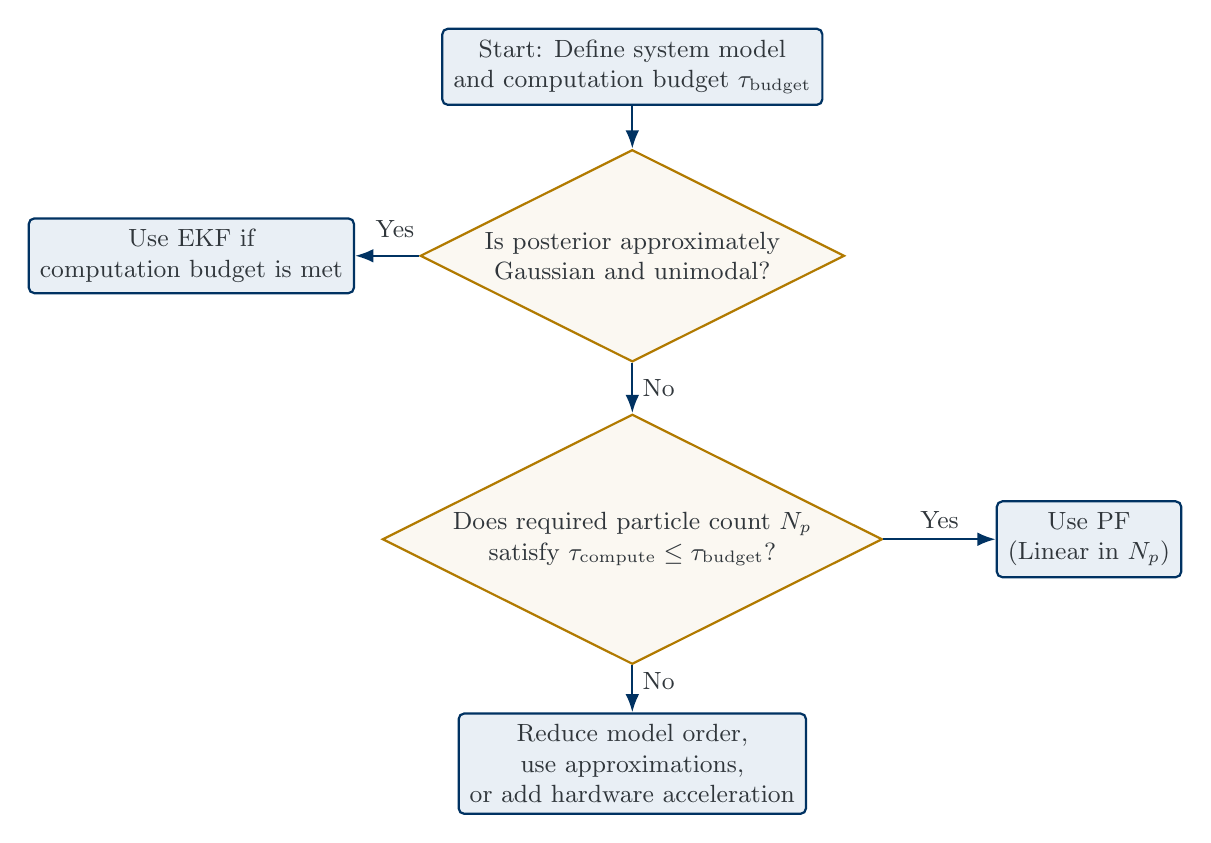
\begin{tikzpicture}[font=\small, text=BookInk, draw=BookBlue, line width=0.8pt, >=Latex,
    node distance=1.6cm,
    every node/.style={font=\small},
    decision/.style={diamond, draw=BookGold, fill=BookGold!5, aspect=2, align=center, inner sep=2pt},
    block/.style={rectangle, draw=BookBlue, fill=BookLight, align=center, rounded corners=2pt, inner sep=4pt},
    line/.style={->, draw=BookBlue, line width=0.8pt}
]

% Nodes
\node[block] (start) {Start: Define system model \\ and computation budget $\tau_{\text{budget}}$};

\node[decision, below of=start, yshift=-.8cm] (gauss)
{Is posterior approximately \\ Gaussian and unimodal?};

\node[decision, below of=gauss, yshift=-2cm] (deadline)
{Does required particle count $N_p$ \\ satisfy $\tau_{\text{compute}} \le \tau_{\text{budget}}$?};

\node[block, left of=gauss, xshift=-4cm] (ekf)
{Use EKF if \\ computation budget is met};

\node[block, right of=deadline, xshift=4.2cm] (pf)
{Use PF \\ (Linear in $N_p$)};

\node[block, below of=deadline, yshift=-1.25cm] (reduce)
{Reduce model order, \\ use approximations, \\ or add hardware acceleration};

% Arrows
\draw[line] (start) -- (gauss);
\draw[line] (gauss) -- node[above, xshift=1mm, yshift = 1mm] {Yes} (ekf);
\draw[line] (gauss) -- node[right] {No} (deadline);
\draw[line] (deadline) -- node[above] {Yes} (pf);
\draw[line] (deadline) -- node[right, yshift = 1mm] {No} (reduce);

\end{tikzpicture}
\end{document}
